%\documentclass[a4paper,12pt,oneside,draft]{article}
\documentclass[a4paper,12pt,oneside]{article}
\usepackage[english]{babel}
\usepackage[utf8]{inputenc}
\usepackage{amsmath}
\usepackage{graphicx}
\usepackage[colorinlistoftodos]{todonotes}

\usepackage{listings}


\usepackage{times}
\usepackage{graphicx}
\usepackage{subfigure}
\usepackage{csvsimple}
\usepackage{color}
\usepackage{url}
\usepackage{hyperref} 
\usepackage{cleveref}
\usepackage{comment}
\usepackage{booktabs}
\usepackage{color}

%Variables macros
\newcommand{\DefineVar}[2]{%
  \expandafter\newcommand\csname var-#1\endcsname{#2}%
} 
\newcommand{\var}[1]{\csname var-#1\endcsname}

\usepackage{courier}
\newcommand{\mono}[1]{\texttt{#1}}
%\newcommand{\mono}[1]{\texttt{\textbf{#1}}}

\title{Modelling and simulation of Lego Mindstorms Motors} 
\author{Elena Tumanov, Antonio Sciarretta, Davide Todeschi}

\date{\today}

\begin{document}

%\maketitle
\makeatletter  % populates \@title, \@author, \@date
\begin{titlepage}
      \centering
      ~~~~~~~~~~~~~\\[-10mm]
      
\includegraphics[keepaspectratio=true, width=8cm]{logounitn.jpg} \\[11mm]

     {
     \large \bfseries Laboratory of Applied Robotics\\[3mm]
     }

     %--------------------------------
     % Set the title, author, and date
     % 

     \vspace{0.5cm}
     {
     \Large \bfseries \textcolor{black}{\@title} \par
     }
     \vspace{1 cm}
     \vspace{1 cm}

     {\large {\@author}}
     \\ \vspace{1 cm}
     \@date

\end{titlepage}

%First part

\section{Introduction}


\subsection{Project goals and steps of implementation} 
We had to implement Modelling and simulation of Lego Mindstorms Motors in 3 steps:
\begin{enumerate}
\item Identification of parameters and control of SISO systems for Lego Motors;
\item Control Design and Digital Implementation of the controller;
\item Modelling and simulation of the larger system, application on the comprehensive model and implementation of digital controller for the whole system.
\end{enumerate}

\subsection{General information about LEGO MINDSTORMS Education}
LEGO MINDSTORMS Education is the next generation in educational robotics, enabling students to discover Science, Technology, Engineering and Mathematics in a fun, engaging, hands-on way. By combining the power of the LEGO building system with the LEGO MINDSTORMS Education technology, teams of students can design, build, program, and test robots. Working together on guided and open-ended engineering projects, the team members develop creativity and problem-solving skills along with other important mathematics and science knowledge. Students also become more skilled in communication, organization and research, which helps prepare them for future success in higher levels of schooling and in the workplace. \\ LEGO MINDSTORMS Education features an advanced 32-bit computer controlled NXT brick, Interactive Servo Motors, Sound, Ultrasonic and other sensors, Bluetooth communication and multiple downloading capabilities. The icon-based LEGO MINDSTORMS Education NXT Software is built on the LabVIEW™ software from National Instruments, an industry standard with applications in many engineering and research fields. \footnote{Lego Mindstorms NXT - Wikipedia, the free encyclopedia, \url{https://en.wikipedia.org/wiki/Lego_Mindstorms_NXT}}.



\section{Used tools}
\subsection{nxtOSEK}
nxtOSEK is an open source platform for LEGO MINDSTORMS NXT. nxtOSEK consists of device driver of leJOS NXJ C/Assembly source code,TOPPERS/ATK (Automotive Kernel, formerly known as TOPPERS/OSEK) and TOPPERS/JSP Real-Time Operating System source code that includes ARM7 (ATMEL AT91SAM7S256) specific porting part, and glue code to make them work together. 
\\
item nxtOSEK can provide:

\begin{itemize}
\item ANSI C/C++ programming environment by using GCC tool chain;
\item C API for NXT Sensors, Motor, and other devices;
\item C++ API for NXT Sensors and Motor which include many third party sensors;
\item TOPPERS/ATK provided real-time multitasking features proven in automotive industry;
\item TOPPERS/JSP provided real-time multitasking features complied with Japan original open RTOS specification ITRON 4.0;
\item Fast execution and less memory consumption (nxtOSEK program is executed natively on the ARM7 and nxtOSEK itself consumed totally just about 10Kbytes).
\footnote{nxtOSEK, \url{http://lejos-osek.sourceforge.net/whatislejososek.htm}}
\end{itemize}

\subsection{ScicosLab}
ScicosLab is a free open-source software package for scientific computation. ScicosLab includes a fork of Scilab, based on Scilab 4, the modeling and simulation tool Scicos and a number of other toolboxes.
\\
Scilab is an interpreted language specifically developed for matrix based numerical computations. It includes hundreds of general purpose and specialized functions for numerical computation, organized in libraries called toolboxes that cover such areas as simulation, optimization, systems and control, and signal processing. These functions reduce considerably the burden of programming for scientific applications. \footnote{Modeling and Simulation in Scilab/Scicos with ScicosLab 4.4, Stephen L. Campbell, Jean-Philippe Chancelier and Ramine Nikoukhah, Second Edition}


\section{Collecting data from motor}
We used Bluetooth connection to collect data from motor.

\subsection{NXT Brofist directory changes}
At the beginning, we set command Set Power to return the current values of the counter from the motor (degrees). 
In the server part, we sent an input step function and after the power, which was 50, we send more than 1000 commands for multiple times (from power 30 to 70).
\\
Because Bluetooth connection is very slow, we chose the following way:
\begin{itemize}
\item We created a buffer in the client part, which has the capacity to store 1000 packets/commands (Set power commands).
\item Stored simultaneously all set power commands and after elaborated all at once.
\item Between the execution of two successive commands we set a wait time of 2 ms.
\item After the execution, we sent back all the results.
\item Set power instructions returned the current values.
\end{itemize}
We modified the packets to add the information about the time.


\subsection{Collecting data through Bluetooth }
Client side modifications:
\\
Added Buffer to store a huge number of instructions. This let us to use Bluetooth only twice per experiment.
\\
Implemented the interface to return also the current measure NXT timestamp.
\\
Modified Set power commands, to return information about current counter and time.
\\
 Server side modifications:
\\
 Implement the interface to include also the current measure NXT timestamp. 
\\
Created Set power commands, which gave a step function with Power 50. 
\begin{enumerate}
\item Send message from PC via Bluetooth to brick that define motor power(that determines the speed).
\item Waited for the elaboration.
\item Receive message from brick with time, input power, tachometer count.
\item Elaborated the speed. 	
\begin{equation}
\Speed Speed = \frac{\text{Count-PrevCount}}{\text{Time–PrevTime}}*\frac{\pi}{180}
\end{equation}
\item We saved data in .csv files that contains information received from the brick. We collected the following information: time, input power, tachometer count, speed(1).
\end{enumerate}

Code is here: \href{https://github.com/etumanov/AppliedRoboticsUNITN/tree/master/DeliverableNI}{Collect Data Implementation}\\
Collected data files are here: \href{https://github.com/etumanov/AppliedRoboticsUNITN/tree/master/DeliverableNI}{Files with Data}

\section{Filtering data and estimating the parameters}
To estimate the parameters we filtered the data using Chebyshev 2 filter and after this we estimated the parameters using a regular method proposed during the course.
\subsection {Filtering}
\subsubsection {Chebyshev 2 filter}
We used Chebyshev 2 filter of order 1 and a cut-off frequency of 0.04.
In the following \cref{fig:D11}., you can see the comparison between Raw Data and Filtered Data for the Power 40.

\begin{figure}[h]%
	\centering
	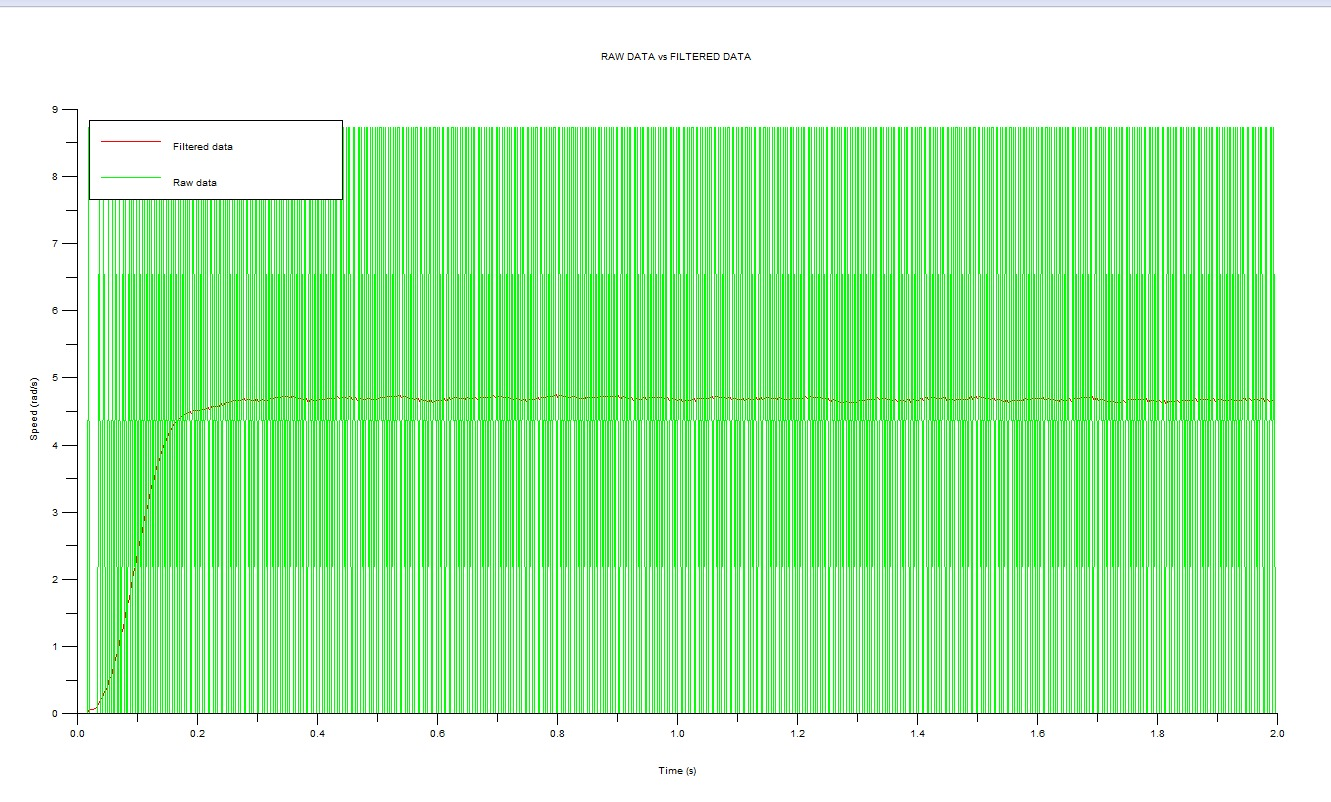
\includegraphics[keepaspectratio=true, width=15cm]{D11.jpg}
	\caption{Raw Data and Filtered Data at Power 40}%
	\label{fig:D11}%
\end{figure}


\subsubsection {Chebyshev instead of Butterworth}

Chebyshev equal ripple magnitude have a better rate of attenuation beyond the pass-band than Butterworth but is considerably more ringing in step response than Butterworth.
This filter response has the steeper initial rate of attenuation beyond the cutoff frequency than Butterworth.This advantage comes at the penalty of amplitude variation(ripple) in the pass-band. Unlike Butterworth and Bessel response, which have 3dB attenuation at the cutoff frequency,Cebyshev cutoff frequency is defined as the frequency at which the response falls below the ripple band. For even-order filters, all riple is above the dc-normalized passband gain response, so cutoff is at 0dB. For odd-order filters, all riple is below the dc-normalized passband gain response, so cutoff is at -(ripple) dB. For a given number of poles, a steeper cutoff can be achieved by allowing more pass-band ripple. The Chebyshev has more ringing in its pulse response than the Butterworth - especially for high-ripple designs.
\\
 Butterworth filter have some overshoot and ringing in step response. This filter has the flattest possible pass-band magnitude response. Attenuation is -3dB at the design cutoff frequency. Attenuation beyond the cutoff frequency is a moderately steep -20dB/decade/pole. The pulse response of the Butterworth filter has moderate overshoot and ringing.
\\
The Butterworth filter is completely defined mathematically by 2 parameters: Cutoff frequency and number of poles. The Chebyshev filter has a third parameter: Passband Ripple.

\subsection {Parameter Estimation}
We need to estimate 3 parameters $q$, $\omega_{n}$, $\xi$. You can find code in 
\\
 \href{https://github.com/etumanov/AppliedRoboticsUNITN/tree/master/DeliverableNI}{Deliverable 1}

We used the following formulas:
\begin{equation}
q = \text{Last speed value}
\end{equation}
\begin{equation}
\xi = \sqrt{\frac{\log(\text{overshot}) ^ 2}{\pi ^ 2 + \log(\text{overshot}) ^ 2}}
\end{equation}
\begin{equation}
\omega_{n} =  \frac{\log(\frac{alpha}{100}) -\log(\frac{1}{\sqrt{1-\xi^2}})}{-\text{settling time} * \xi}
\end{equation} 

We started evaluation from Steady state values of the filtered functions (f - filtered function).

\begin{enumerate}
\item Steady state value estimation = $k_{est}$;
\begin{equation}
k_{est} = \frac{\text{f}}{{input signal }}
\end{equation}
We evaluated the damping factor $\xi$, called $\xi${est}.

\begin{equation}
\xi_{est} = \sqrt{\frac{\log(\text{overshot}) ^ 2}{\pi ^ 2 + \log(\text{overshot}) ^ 2}}
\end{equation}


\item Natural frequency $\omega_{n}$ which is called  $\omega_{nest}$.

\begin{equation}
\omega_{nest} =  \frac{\log(\frac{alpha}{100}) -\log(\frac{1}{\sqrt{1-\xi^2}})}{-\text{settling time} * \xi_{est}}
\end{equation}
Where: alpha= 3;


\item Made the estimations of our system using the following estimation formula:

\begin{equation}
G_{est} =  \frac {\text .{k_{est}}} {\frac{s^2}{\omega_{n}^2} + 2* {\frac {\xi_{est}}{\omega_{nest}}*s+1}}
\end{equation}

We evaluated all previous values for 40 times from Power 30 to Power 70 and we made the mean of the values.\\ [5 mm]
Result values are: \\ [5 mm]
\begin{equation} 
k_{est} = 0.1531618 (Steady state value) \\
\end{equation}
\begin{equation}
\xi_{est}= 0.8209478 (Damping factor) \\
\end{equation}
\begin{equation}
\omega_{nest}= 16.515118 (Natural frequency) \\ 
\end{equation}


In the following \cref{fig:D12}., you can see the difference between Estimation and Test for Power of 40, 50 and 60.

\begin{figure}[h]%
	\centering
	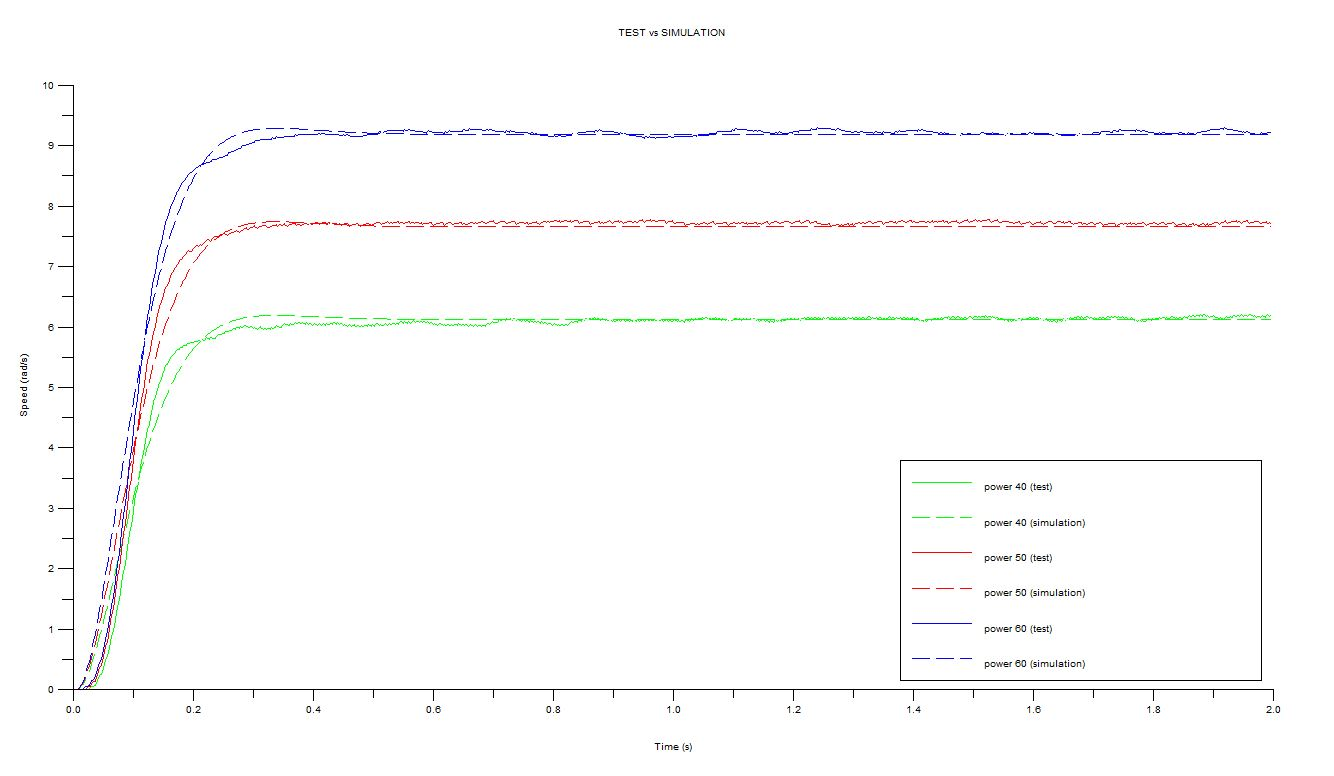
\includegraphics[keepaspectratio=true, width=15cm]{D12.jpg}
	\caption{Test vs Simulation (Power 40, 50, 60)}%
	\label{fig:D12}%
\end{figure}


\subsection {Performance indices to control system}
A metric is needed to measure distances between observed and predicted data and, hence, to assess model fit. As a metric, we adopted some standard indices used as performance indices for control systems.
\\ The indices formulas: \\ 
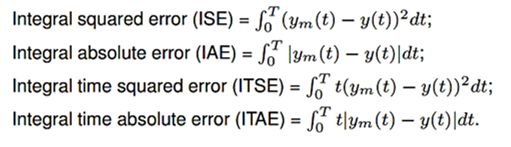
\includegraphics[keepaspectratio=true, width=10cm]{formulas1.png} 

We tested our system three times with Power 40, Power 50 and Power 60. \\

Got the following errors calculating the average value of the above formulas:\\
Power 40: AverageError = 38.2590 \\
Power 50: AverageError = 53.2616 \\
Power 60: AverageError = 45.9473 \\

Mean squared error: \\
Power 40: MSE = 0.0259 (rad/s)^2 \\
Power 50: MSE = 0.0324 (rad/s)^2 \\
Power 60: MSE = 0.0408 (rad/s)^2 \\


Used filter caused the big error at the beginning of the axis in the following figure because it have a big delay.
\\
In the following \cref{fig:D13}., you can see the difference between Output Estimations and Input Estimations for Power of 40, 50 and 60. \\
\begin{figure}[h]%
	\centering
	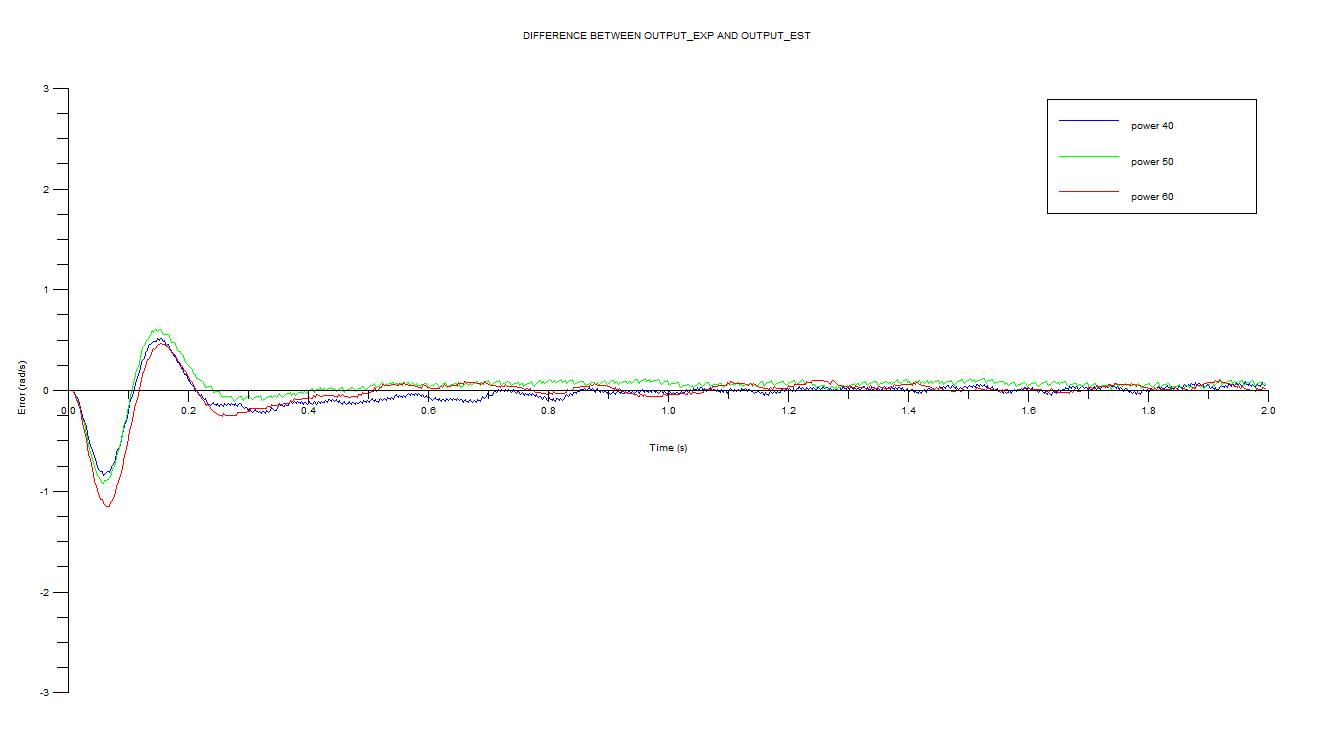
\includegraphics[keepaspectratio=true, width=15cm]{D13.jpg}
	\caption{Difference between Input and Output estimations}%
	\label{fig:D13}%
\end{figure}

\section{General description of Control Design}
Control Design and Digital implementation of controller for the Lego NXT motor.
The second task was to show our designed controller, describe it properties and digital implementation.
\subsection {General information about Control design for the motor}

Root locus: In control theory and stability theory, root locus analysis is a graphical method for examining how the roots of a system change with variation of a certain system parameter, commonly a gain within a feedback system. This is a technique used as a stability criterion in the field of control systems developed by Walter R. Evans which can determine stability of the system. The root locus plots the poles of the closed loop transfer function in the complex S plane as a function of a gain parameter (see pole–zero plot). \footnote{Root Locus,\url{https://en.wikipedia.org/wiki/Root_locus}} \\

Closed-loop transfer function: in control theory is a mathematical expression (algorithm) describing the net result of the effects of a closed (feedback) loop on the input signal to the circuits enclosed by the loop. \footnote{Closed loop transfer function,\url{https://en.wikipedia.org/wiki/Closed-loop_transfer_function }}
\footnote{Root locus course,\url{http://disi.unitn.it/~palopoli/courses/ECL/RootLocus.pdf}}\\

In such a case, we have the plant P(s) and an additional block C(s): the controller. The objective was to determine C(s) in order to satisfy certain closed loop performance.

\begin{figure}[h]%
	\centering
	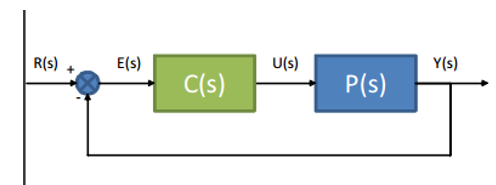
\includegraphics[keepaspectratio=true, width=10cm]{closedloop.png}
	\caption{Closed loop}%
	\label{fig:closedloop}%
\end{figure}

\section{Control design for the motor}
\subsection{Needed performance}
\begin{itemize}
\item Steady state tracking error = 0
\item Overshot $<$ 20\%
\item Settling time $<$ 0.2s
\end{itemize}
Overshot requirement on root locus plot is shown by the following formula:
\begin{equation}
\frac{-{\pi}{\xi}}{\sqrt{1-\xi^{2}}} <= \frac{log^2{0.2}}{\pi} = \alpha
\end{equation}

% show settling time requirement, it is possible to use the dominant pool approximation:
%\begin{equation}
%\Re = \frac{ln(\alpha)}{0.4}
%\end{equation}

\subsubsection{Closed loop system}
\begin{enumerate}
\item Closed loop system: \\

\begin{equation}
Gcl = \frac{K_{c}*C*G}{1 + K_{c}*C*G}
\end{equation}
 
\item Set  \\
\begin{equation} 
K_{c} = 1 ; \\
C = 1
\end{equation} 

\item Added a pole \\
\begin{equation} 
C = 1/s 
\end{equation} 
to obtain 0 steady state error, possible due to Internal model principle.
\end{enumerate}

\subsection{Our Motor Design}
\begin{equation}
C(s) = \frac{(s+10)^2}{s*(s+31)}
\end{equation}
\begin{equation}
K_{c} = 12
\end{equation}



Root locus is illustrated in \cref{fig:D22}, and the response to the step function in \cref{fig:D21}.\\ 
Results of Scicoslab simulation \cref{fig:D23} are shown in the following figures:
\begin{itemize}
\item $\Omega$ in \cref{fig:D25}
\item Power in \cref{fig:D24}
\end{itemize}
Code is in this directory.\footnote{\url{https://github.com/etumanov/AppliedRoboticsUNITN/tree/master/DeliverableNII }}.

\begin{figure}
	\centering
	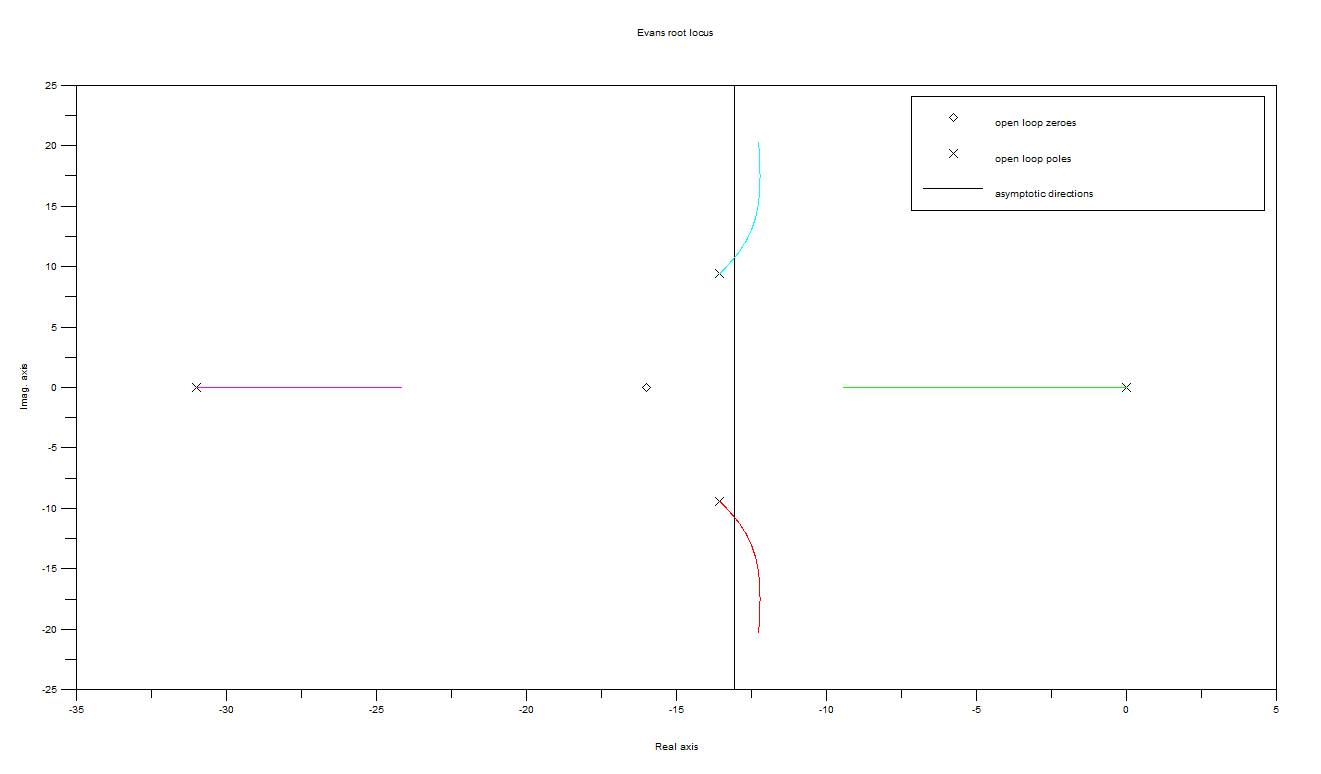
\includegraphics[width=\columnwidth]{D22.jpg}
	\caption{Root locus}
	\label{fig:D22}
	\centering
	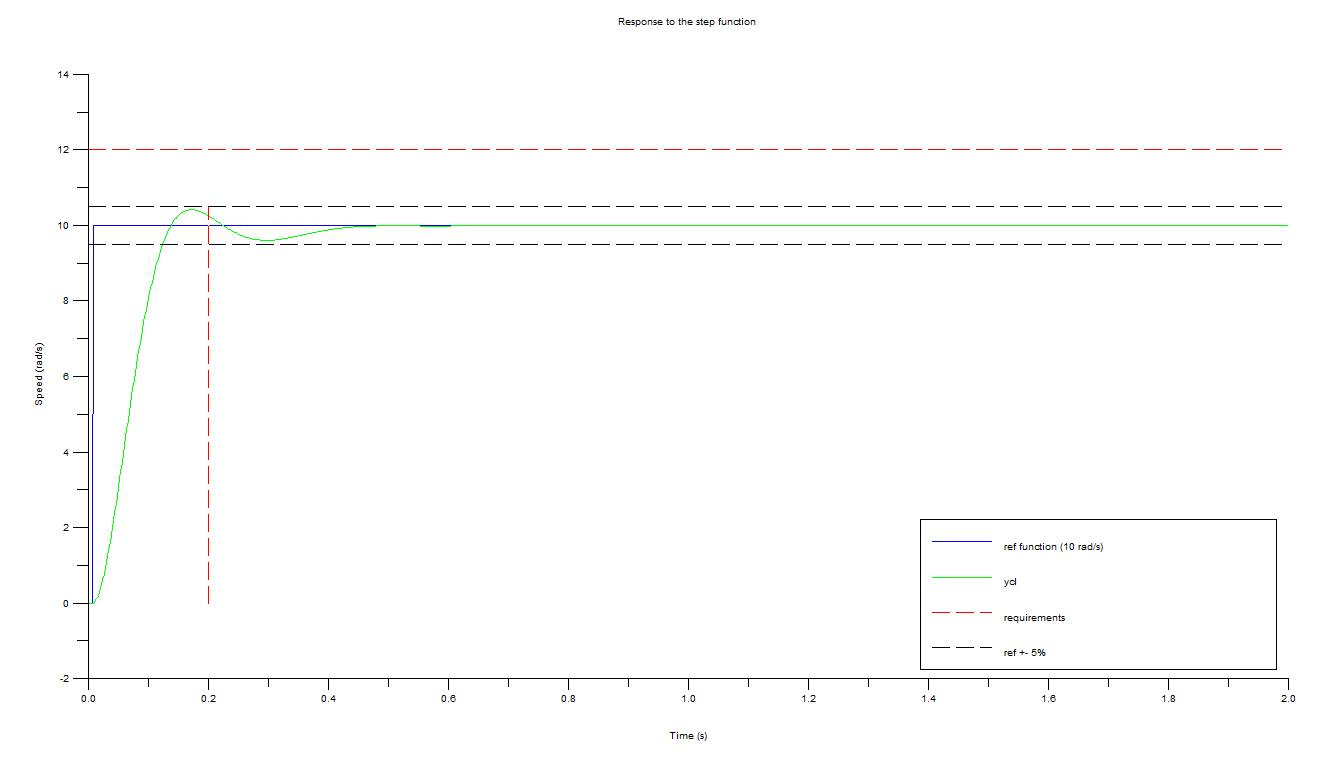
\includegraphics[width=\columnwidth]{D21.jpg}
	\caption{Response to the step function}
	\label{fig:D21}
\end{figure}

\begin{figure}
	\centering
	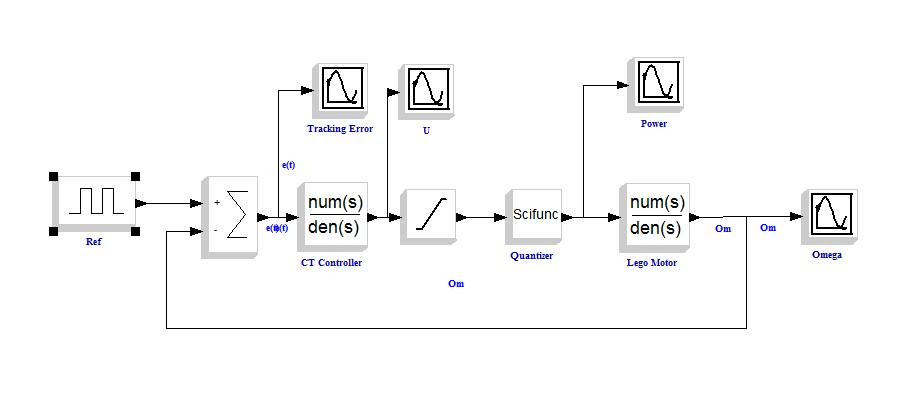
\includegraphics[width=\columnwidth]{D23.jpg}
	\caption{Controller Design}
	\label{fig:D23}
\end{figure}

\begin{figure}
	\centering
	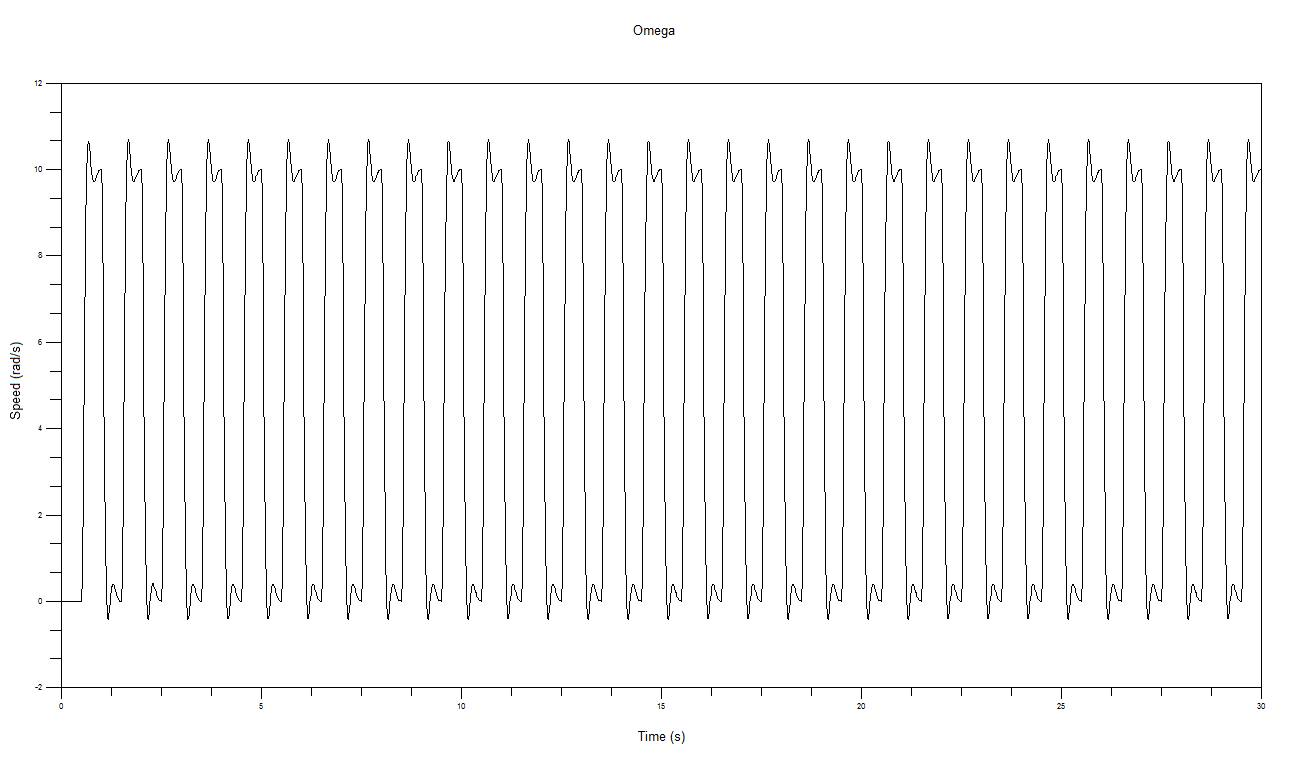
\includegraphics[width=\columnwidth]{D25.jpg}
	\caption{Speed $\Omega$}
	\label{fig:D25}
\end{figure}
\begin{figure}
	\centering
	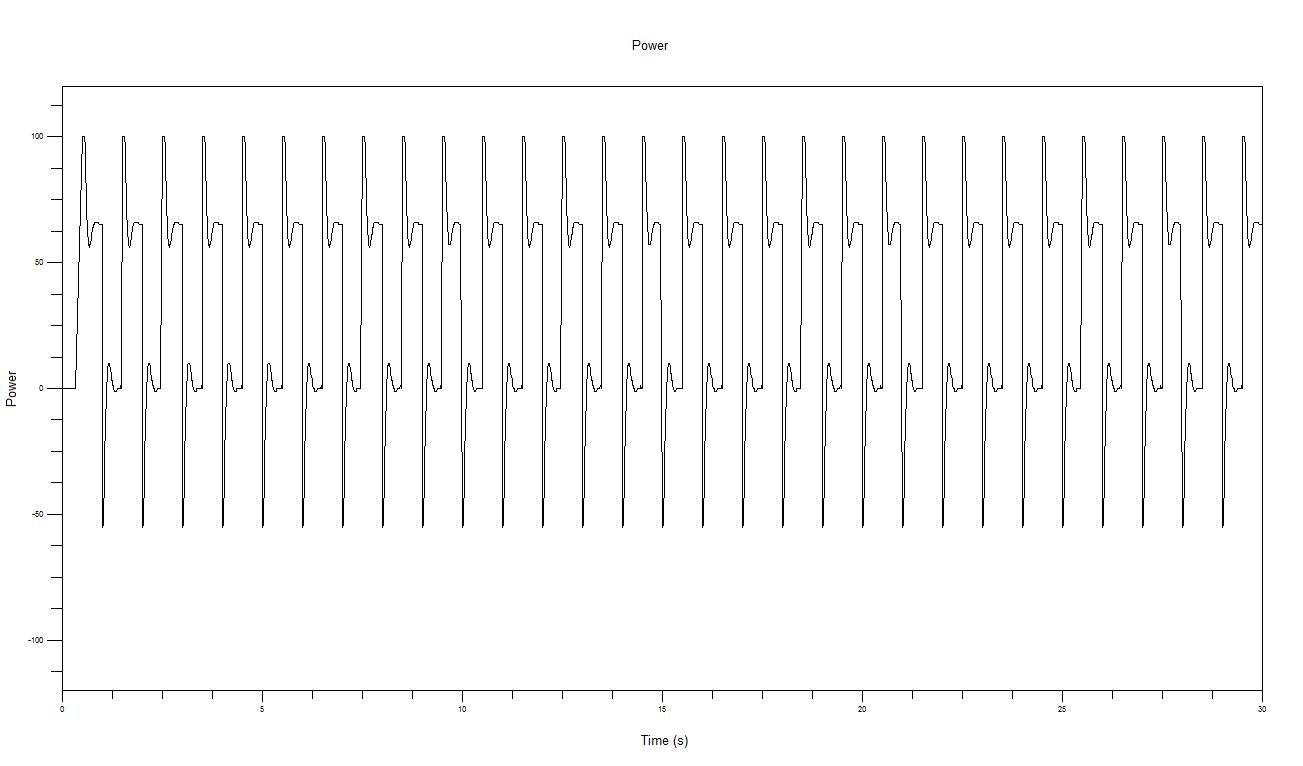
\includegraphics[width=\columnwidth]{D24.jpg}
	\caption{Power}
	\label{fig:D24}
\end{figure}


\section{Digital implementation of the controller}

\begin{figure}
	\centering
	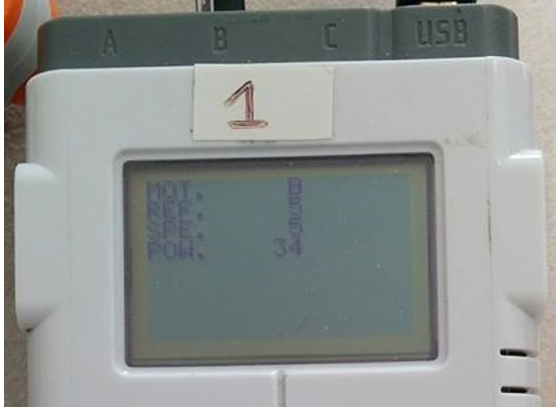
\includegraphics[width=\columnwidth]{task2.png}
	\caption{Brick with REF, SPE and POW values}
	\label{fig:task2}
\end{figure}

What we have done is \cref{fig:task2}: \\
\begin{itemize}
\item Set a speed we want to reach (REF) \\
\item Evaluated the current speed (SPE) \\
\item Calculated the power we need (POW)
\end{itemize}

\begin{multline}
y_{k+2} = \frac{1}{-31 * sT - 2} (-4 * y1 +(-31 * sT + 2) * y0 + gain * (u2*(-128*sT*sT - 32*sT -2) \\
+u1*(4-256*sT*sT)+u0*(-128*sT*sT+32*sT-2)))
\end{multline}
Speed estimated using Exponential moving average:
S_1 = Y_1, t>1  \\
\begin{equation}
\centering
S_{t} = \alpha \cdot Y_{t} + (1-\alpha) \cdot S_{t-1}
\end{equation}

Code is available in a shared folder\footnote{\url{https://github.com/etumanov/AppliedRoboticsUNITN/tree/master/DeliverableNII}}.

\section{Modelling and simulation of the larger system}
Our last task was to Model and simulate a larger system:
\begin{enumerate} 
\item 2 motors;
\item Moving straight(no deviations) without any visual or position control, but only using the the implementation of a digital controller for two motors;
\item Implementing an additional controller which is evaluating the error of the speed from the first and second motor in order to adjust them;
\item Test on the Lego Mindstorms Robot for 3 different distances and 3 different speeds.
\end{enumerate} 
Our actions:
\begin{enumerate} 
\item Modified the packets which contain the information about the distance;
\item In the client we modified the command set speed;
\item Duplicating the command and controller to the both the motors;
\item Add the control on the distance (for the distance you can add the formula, the one in the code);
\item Add the controller on the angle omega which has to be 0.

\end{enumerate} 


\begin{figure} [h]%
	\centering
	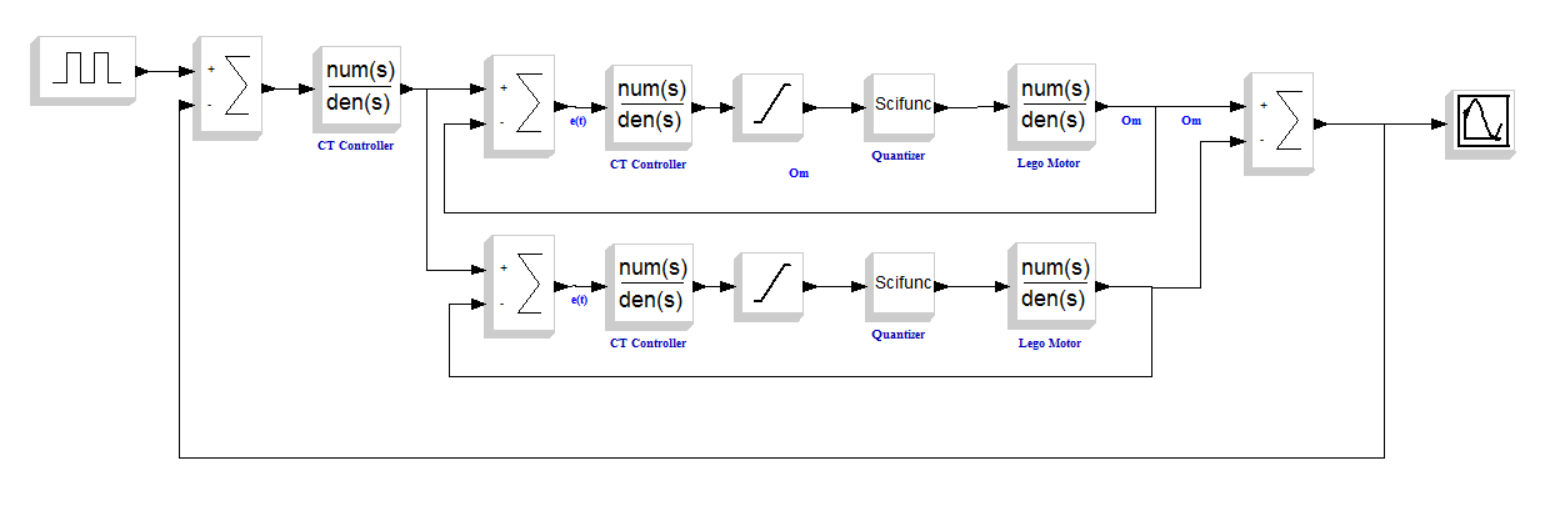
\includegraphics[width=\columnwidth]{completesystem.png}
	\label{fig:completesystem}
	\caption{Complete System} %
\end{figure}

%New colors defined below
\definecolor{codegreen}{rgb}{0,0.6,0}
\definecolor{codegray}{rgb}{0.5,0.5,0.5}
\definecolor{codepurple}{rgb}{0.58,0,0.82}
\definecolor{backcolour}{rgb}{0.95,0.95,0.92}

%Code listing style named "mystyle"
\lstdefinestyle{mystyle}{
  backgroundcolor=\color{backcolour},commentstyle=\color{codegreen},
  keywordstyle=\color{magenta},
  numberstyle=\tiny\color{codegray},
  stringstyle=\color{codepurple},
  basicstyle=\footnotesize,
  breakatwhitespace=false,         
  breaklines=true,                 
  captionpos=b,                    
  keepspaces=true,                 
  numbers=left,                    
  numbersep=8pt,                  
  showspaces=false,                
  showstringspaces=false,
  showtabs=false,                  
  tabsize=2
}

%"mystyle" code listing set
\lstset{style=mystyle}

To evaluate speed of each motor we used this function: \\
 
\begin{lstlisting}[frame=single]  
double evaluate_speed(motor_t * motor, double previousSpeed) {
	double space_rad = (motor->revolutions[0] - motor->revolutions[1]) * (PI / 180.0);
	double speed_rad = space_rad/ (0.002);
	speed_rad = speed_rad * alpha + (1-alpha) * previousSpeed;
	return speed_rad;
\end{lstlisting}
	

To control the speed from the both motors we implemented next function: \\


\begin{lstlisting}[frame=single] 
void updateMotors(engines_t * motors){
	motor_t *motor;
    motor_t *otherMotor;
	for(int m = 0; m < 2; m++){
		switch (m){
			case 0: motor = &(motors->first); otherMotor = &(motors->second); break;
			case 1: motor = &(motors->second); otherMotor = &(motors->first); break;
		}
		for (int i = SAMP_NUM; i > 0; i--){
			motor->revolutions[i] = motor->revolutions[i-1];
			motor->speeds[i] = motor->speeds[i-1];
		}
		motor->revolutions[0] = nxt_motor_get_count(motor->port);
		motor->times[0] = ecrobot_get_systick_ms();
		motor->speeds[0] = evaluate_speed(motor, motor->speeds[1]);
		
		if(motor->speed_control_type == NOT_USING)
			continue;
		
		if(motor->speed_control_type == PID_CONTROLLED){

			double distance = (((motor->revolutions[0] + otherMotor->revolutions[0])/2.0) * PI/180) * 0.028;

			if(abs(distance) >= motor->distance_ref[0]){
				for (int i = 0; i < BUFFER_SIZE - 1; i++){
					motor->speed_ref[i] = motor->speed_ref[i+1];
					motor->distance_ref[i] = motor->distance_ref[i+1];
					otherMotor->speed_ref[i] = otherMotor->speed_ref[i+1];
					otherMotor->distance_ref[i] = otherMotor->distance_ref[i+1];
				}
				motor->speed_ref[BUFFER_SIZE-1] = 0;
				motor->distance_ref[BUFFER_SIZE-1] = 0;
				otherMotor->speed_ref[BUFFER_SIZE-1] = 0;
				otherMotor->distance_ref[BUFFER_SIZE-1] = 0;
			}
			
			if(distance < motor->distance_ref[0]){
				double error = motor->speed_ref[0] - motor->speeds[0];
				double rotationError = rotationController(motors);

				if(m == 0) {
					error = error - rotationError/2;
					motor->powers[0] = controller(error);

				}
				if(m == 1) {
					error = error + rotationError/2;
					motor->powers[0] = controller2(error);
				}

			}
		}
		
		nxt_motor_set_speed(motor->port, motor->powers[0], 1);
	}
}
\end{lstlisting}

Full implimentation of the system can see in \footnote{\url{https://github.com/etumanov/AppliedRoboticsUNITN/tree/master/DeliverableNIII}}. \\ 

\\Bellow is the result from one test: \\

\begin{figure} [h]%
	\centering
	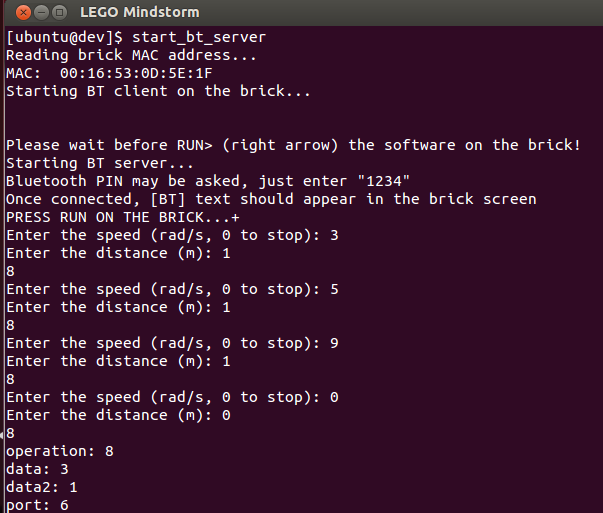
\includegraphics[width=10 cm]{finaltest.png}
	\caption{Introduced Speeds and Distances from terminal} %
\end{figure}

\begin{figure} [h]%
	\centering
	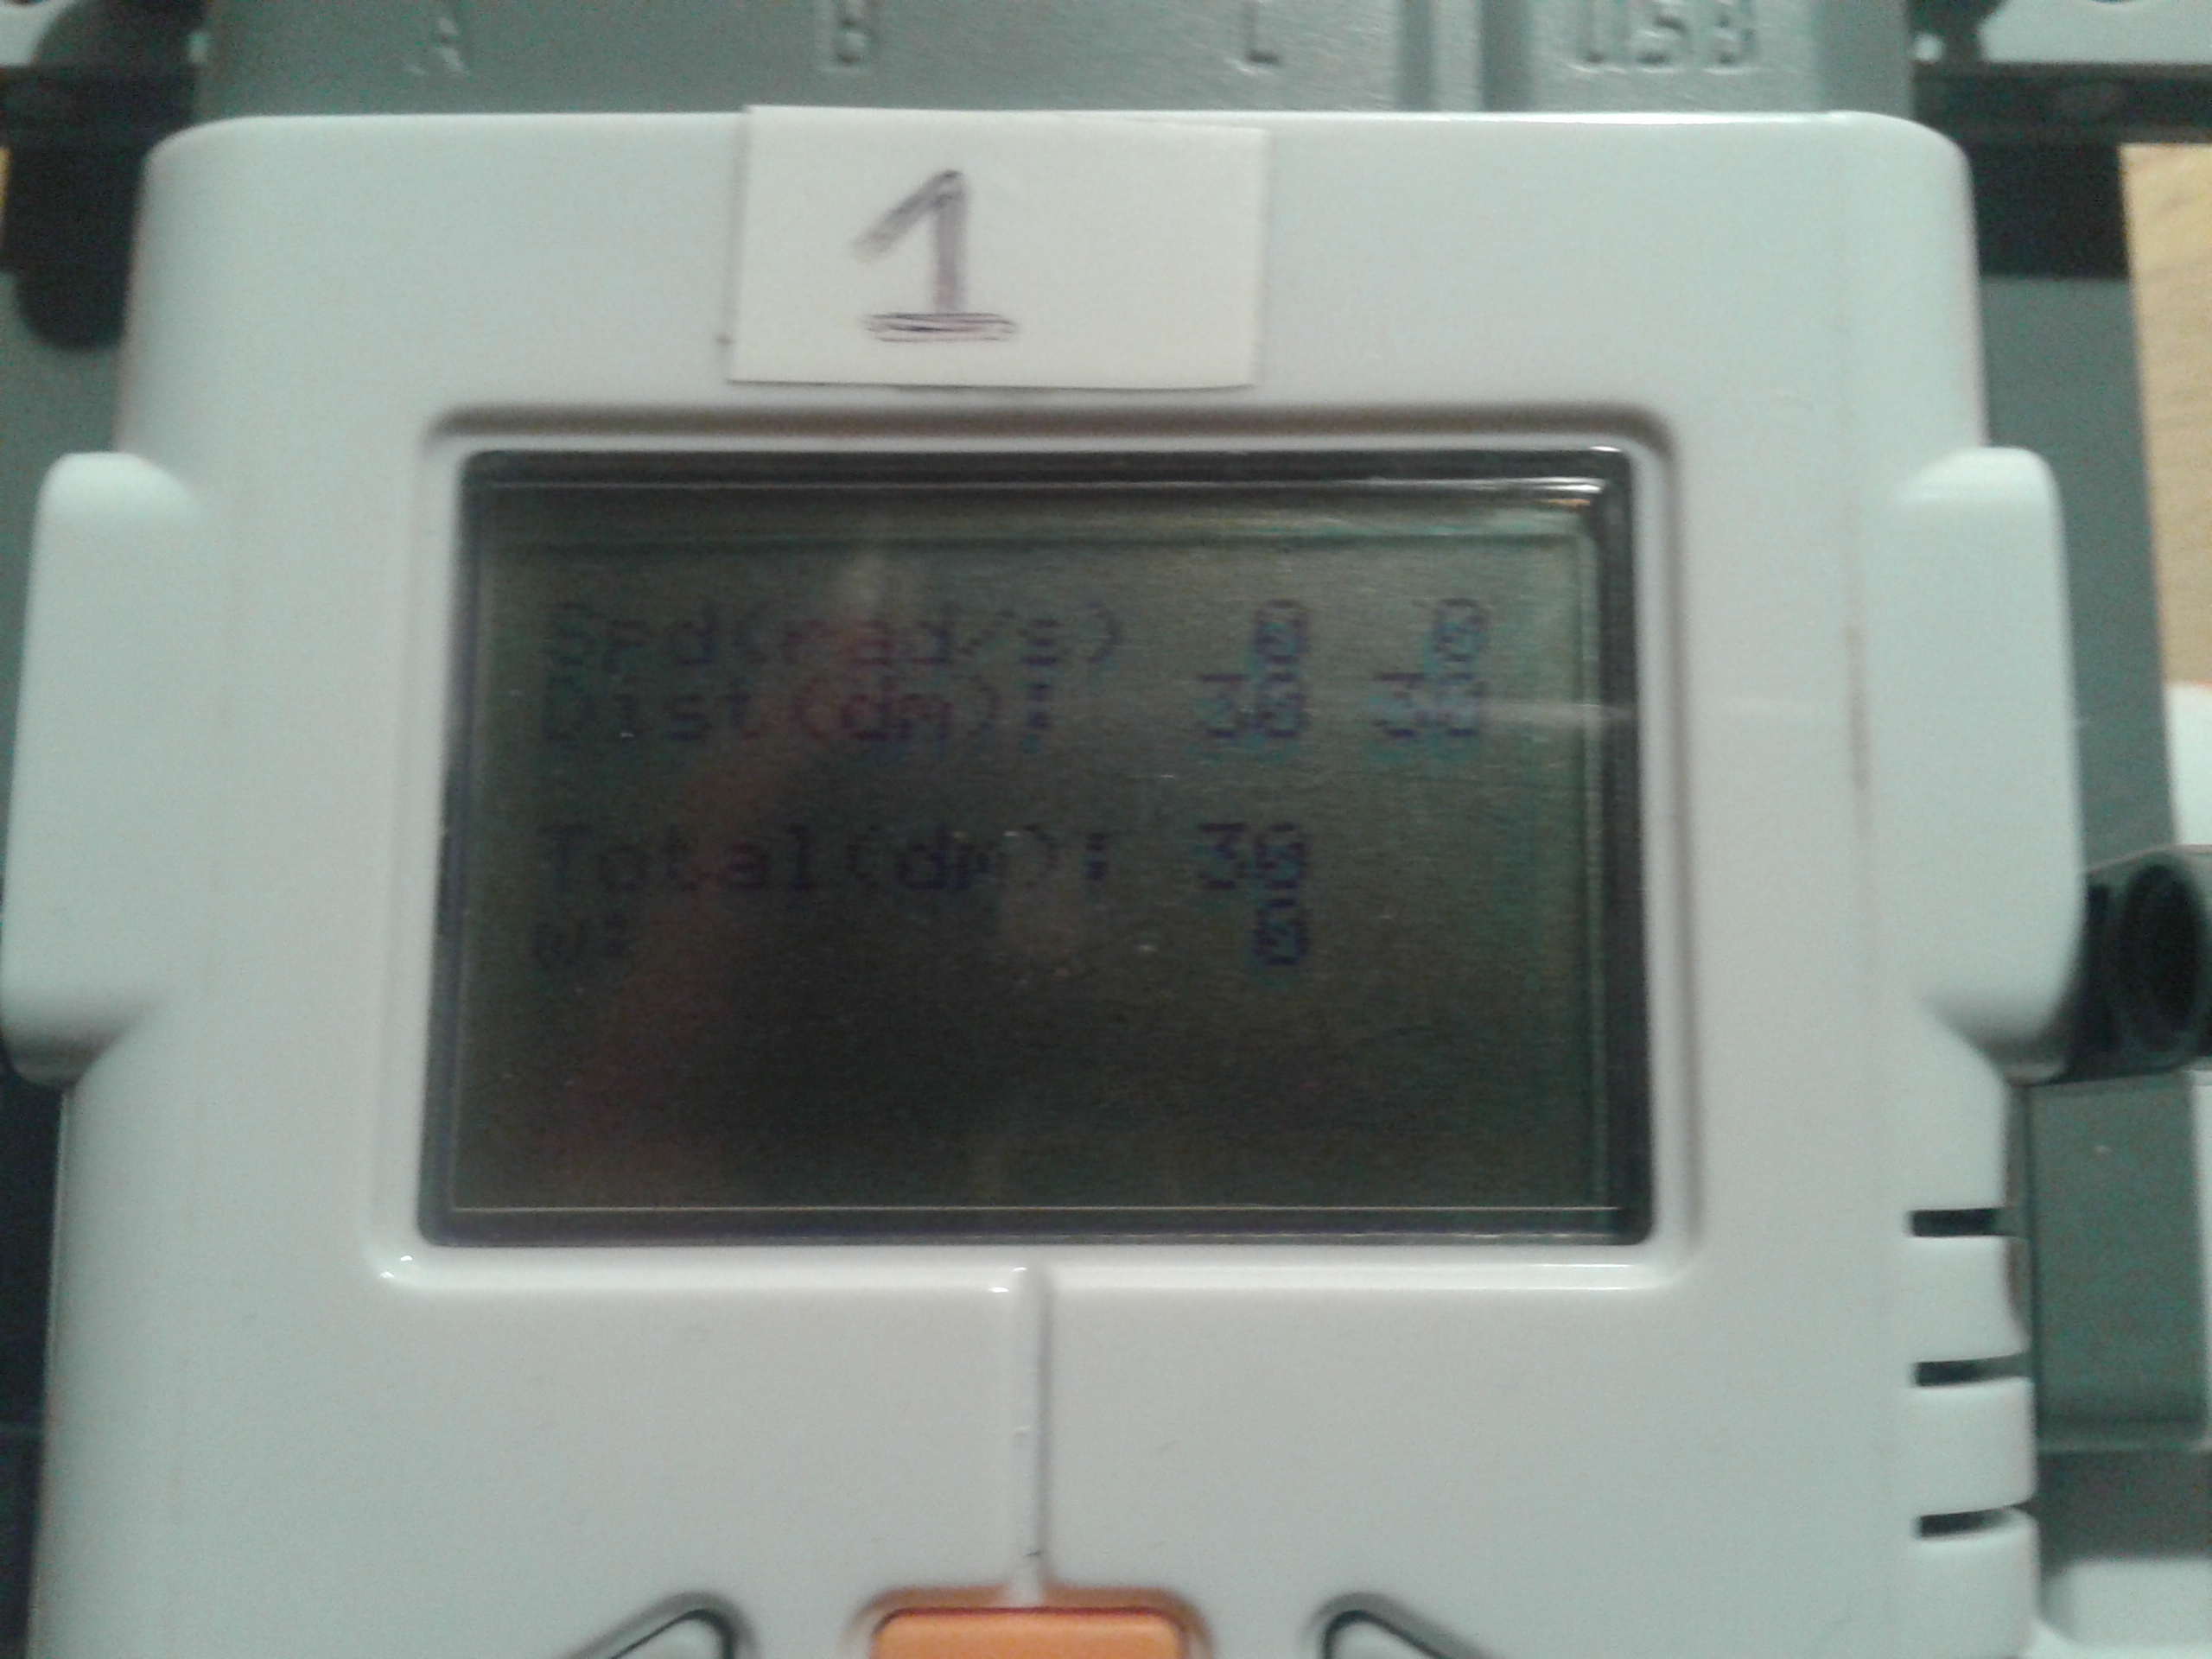
\includegraphics[width=7 cm]{brick1.jpg} 
	\caption{Results on the brick, w = 0 as we expected} %
\end{figure}

\begin{figure}
	\centering
	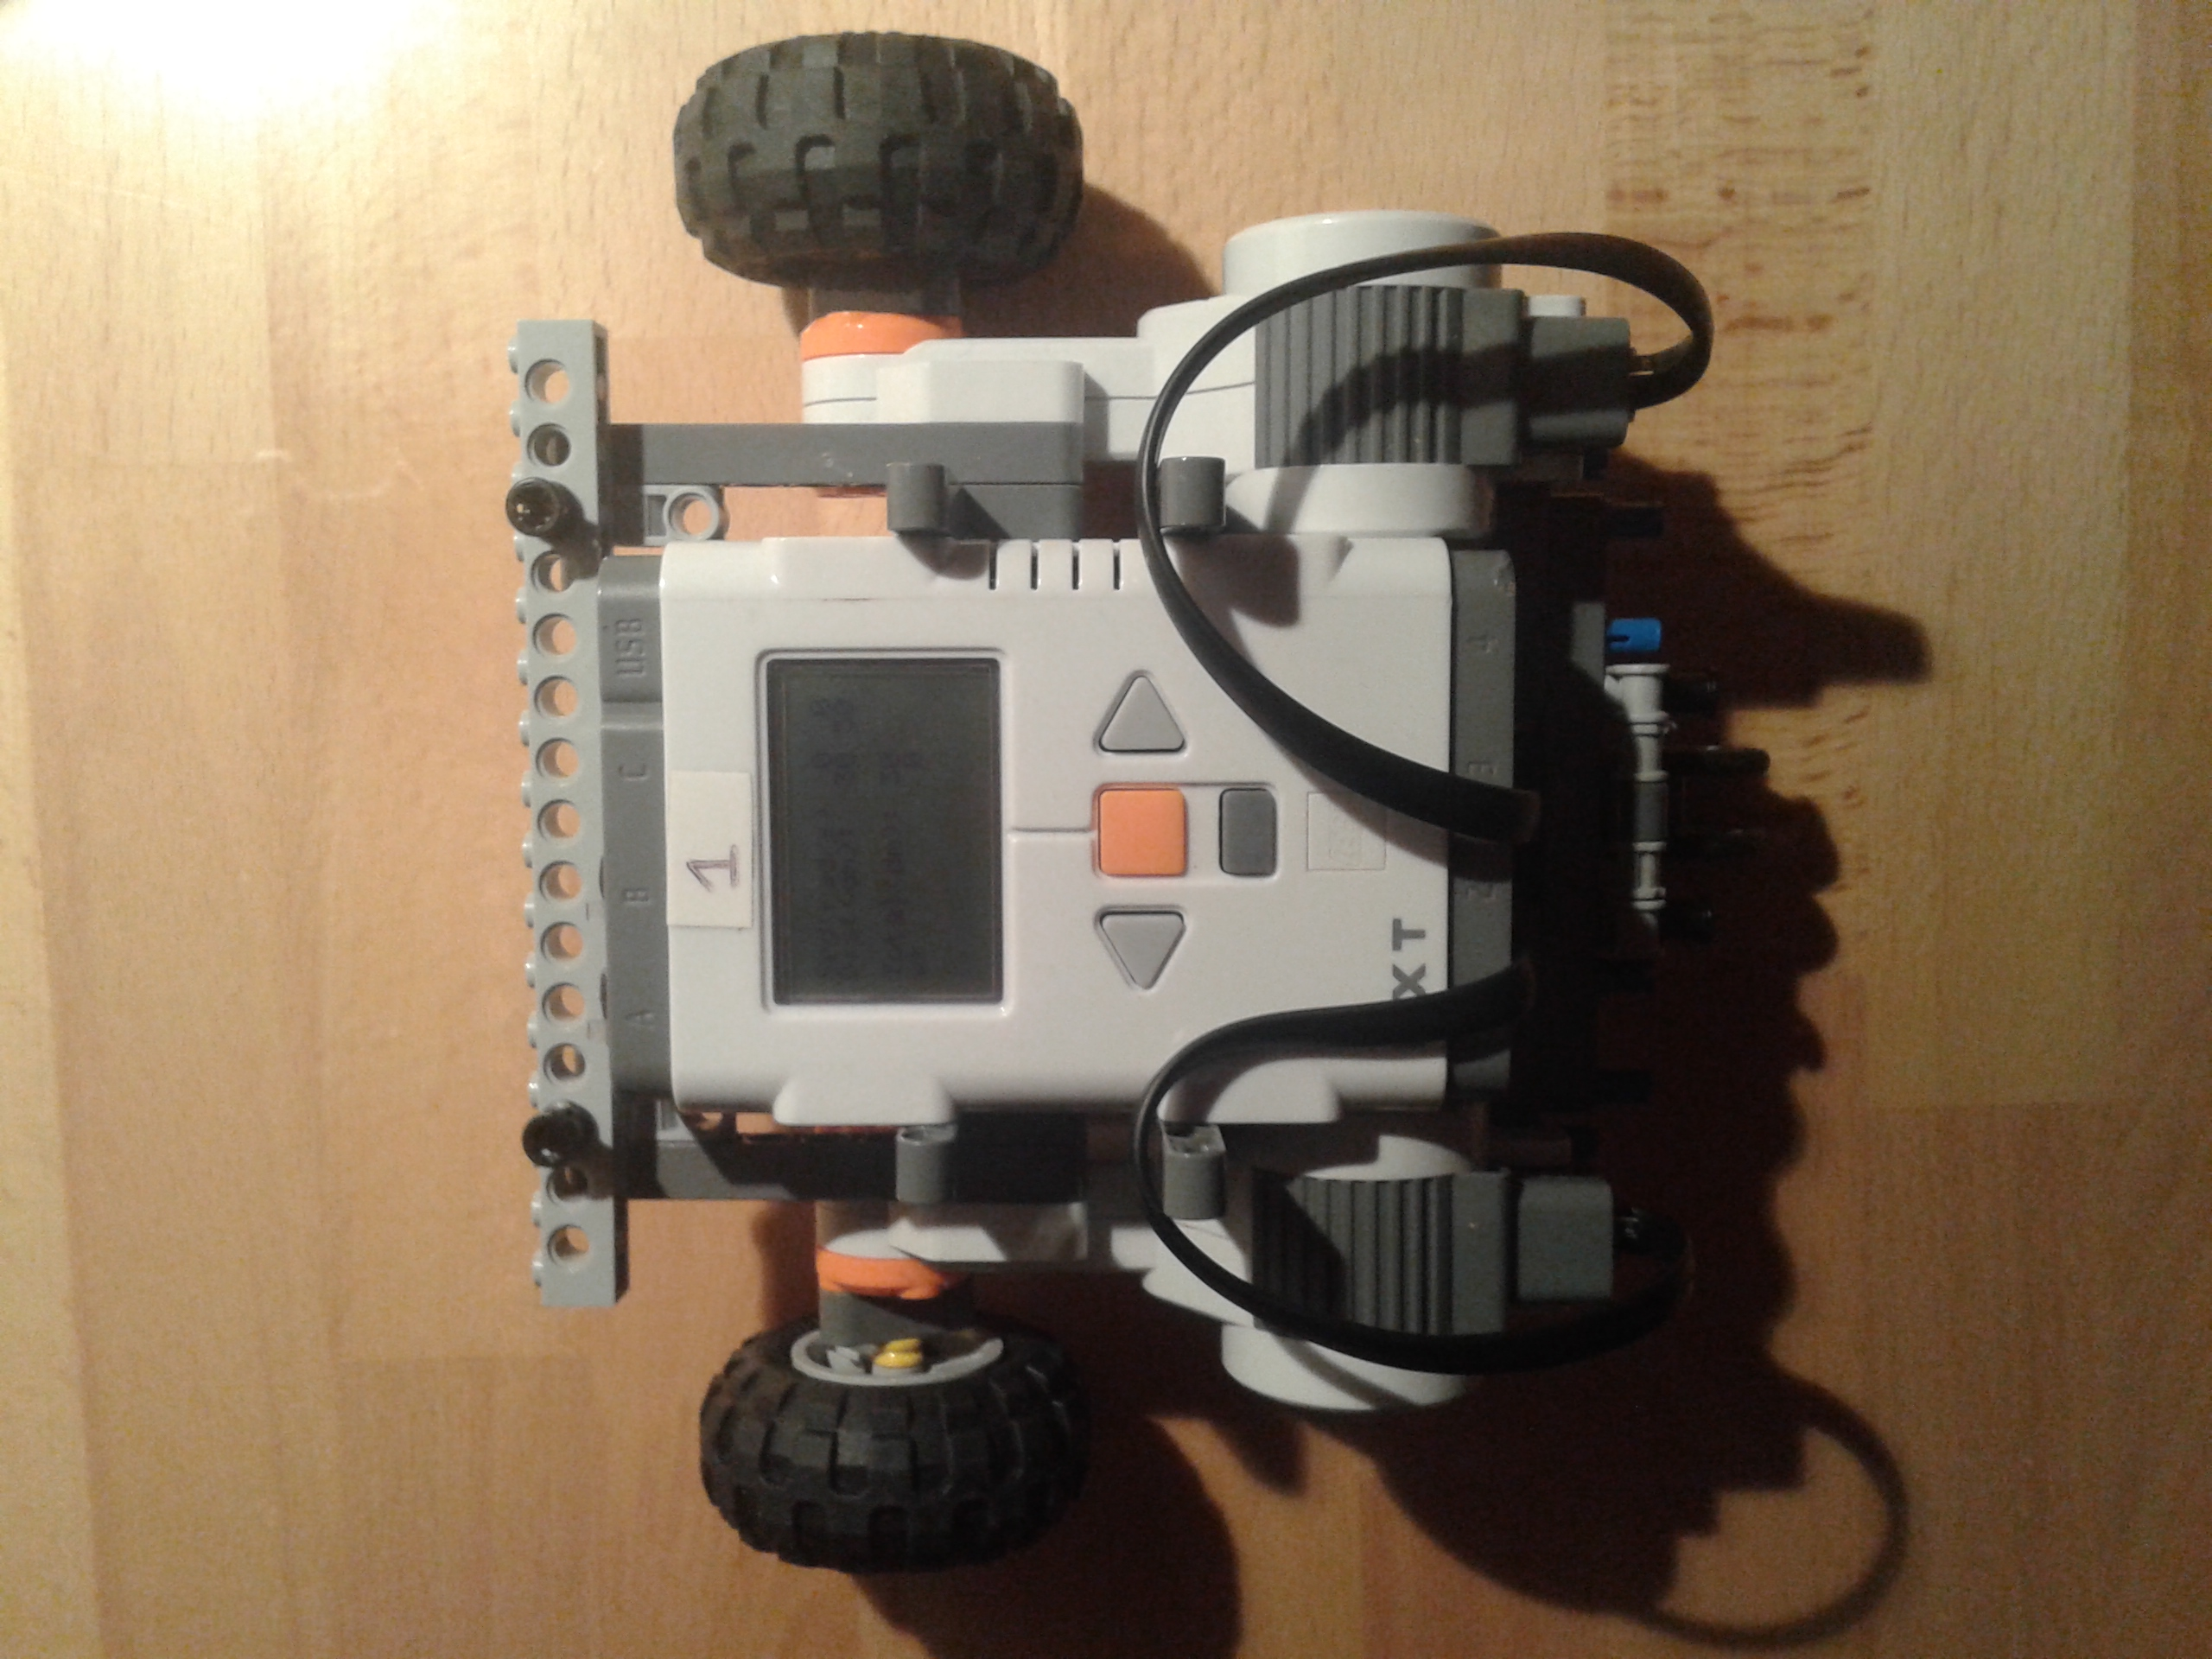
\includegraphics[width=7 cm]{robot.jpg}
	\caption{Our Robot Construction}
\end{figure}


\section{Conclusions}

While working on this project, we applied a lot of knowledge learned at the courses of Laboratory of Applied Robotics. Furthermore, we gained a lot of experience in programming an embedded system. It was very interesting and exciting to implement a real Robot and see the expected results in simulation and SciLab Graphs. \\
The scope of this project was to get familiarity with the overall process of design a complete robotic system.\\
We have subdivide our work in 3 steps: identification phase, controller design and system realization.\\
Above we illustrated our method of identification of parameters from Lego Mindstorms motors based on the collected data. In this phase, we had to solve a lot of different problems; some of them were more technical problems, like understanding and working with NXT C API, bluetooth slowness, communication protocol definition and so on, while others were more theoretical, like model definition, data filtering, estimates evaluation, etc.\\
After some processing, it was possible to compare the predicted behavior of the system with our observation.\\
For the second phase, our goal was to design a controller for the motor and to realize a digital implementation, given some requirements. Here we faced some trouble due to errors in the previous phase: we didn't convert properly some data's units of measurement, therefore we had to recompute all values from the first step. \\
With the theory provided by the study of the root locus, we developed a system which matches the requirements we had. Above we showed how our implementation is properly working.\\
Our last deliverable was to present a complete system which is a tricycle, moving straight. Our system is composed by two independent motors that move as many wheels, and a third free wheel for balancing. In order to implement this we made a stable construction with 2 wheels in front and the third one in the back. We realized two controllers, one for each independent motor, and a third to control the direction. The last one is simply verifying that the overall speed of the two motors is the same (this is the big condition to move straight.\\
This is all the work we had to do in order to realize our simple robot system. Thanks to this project, now we are more conscious about the work that is behind such systems and we have some good intuitions about how to realize them.

\end{document}